% mainfile: ../../main.tex
\chapter{Example applications}\label{ch:ff:examples}
We now present example applications of the software package and the formalism.
As stated before, we focus on the decay amplitudes \decayamps and its associated filter functions and assume that the unitary errors generated by the frequency shifts \freqshifts are either small (as is the case for gate fidelities) or calibrated out.
All of the examples shown below are part of the software documentation as either interactive \jupyter notebooks~\cite{Kluyver2016} or Python scripts.
In the following, we give angular frequencies and energies in units of inverse times (\eg \si{\per\second}) while ordinary frequencies are given in \si{\hertz} and we write $\ev*{\liouvUe(\tau)} = \liouvUe$ for legibility.

\section{Singlet-triplet two-qubit gates}\label{sec:ff:examples:optimized_gates}
In order to benchmark fidelity predictions of our implementation as well as demonstrate its application to nontrivial pulses, we compute the first-order infidelity of the two-qubit gates presented in~\citer{Cerfontaine2020b} and compare the results to the reference's Monte Carlo calculations.
There, a numerically optimized gate set consisting of $\lbrace\XID2,\YID2,\CNOT\rbrace$ for exchange-coupled singlet-triplet spin qubits is introduced, taking into account different noise spectra and realistic control hardware.

For readers unfamiliar with the reference we briefly summarize the physical system and noise model entering the optimization.
The authors consider four electrons confined in a linear array of four quantum dots in a semiconductor heterostructure.
Each electron $i\in\lbrace 1,2,3,4\rbrace$ experiences a different static magnetic field $B_i$ so that there is a gradient $b_{ij} = B_i - B_j$ between two adjacent dots $i$ and $j$.
This gives rise to spin quantization along the magnetic field axis and defines the eigenstates $\lbrace\ketud,\ketdu\rbrace$ that span the computational subspace of a single qubit so that the accessible Hilbert space of the two-qubit system is spanned by $\lbrace\ketud,\ketdu\rbrace^{\otimes 2}$.
The magnitude of the exchange interaction $J_{ij}$ between two adjacent dots $i$ and $j$ is controlled via gate electrodes located on top of the heterostructure that can be pulsed on a nanosecond timescale with an arbitrary waveform generator (AWG).
Changing the gate voltages changes the detuning $\eps_{ij}$ of the electrochemical potential between dots and in turn leads to a change in exchange coupling according to the phenomenological model $J_{ij}(\epsilon_{ij})\propto\exp(\epsilon_{ij})$.

The pulses are defined by a set of discrete detuning voltages $\epsilon_{ij}$ passed to an AWG with a sample rate of \qty{1}{\giga S\per\second} and constant magnetic field gradients $b_{ij}$ are assumed.
To reflect the fact that the qubits experience a different pulse than what is programmed into the AWG due to cable dispersion and non-ideal control hardware, the detunings are convoluted with an experimental impulse response~\cite{Cerfontaine2020b}.
Finally, the signal is discretized as piecewise constant by slicing each segment into five steps, yielding a time increment of $\Delta t = \qty{0.2}{\nano\second}$.

To find optimal detuning pulses, a Levenberg-Marquardt algorithm iteratively minimizes the infidelity, leakage, and trace distance from the target unitary.
For the infidelity, contributions from quasistatic magnetic field noise as well as quasistatic and white charge noise are taken into account during each iteration.
Because treating colored (correlated) noise using Monte Carlo methods is computationally expensive (\cf \cref{sec:ff:performance:complexity}), the infidelity due to fast \oneoverf-like noise is only computed for the final gate and not used during the optimization.

Two-qubit interactions are mediated via the exchange $J_{23}$ that makes the states \ketuudd and \ketdduu accessible.
They constitute levels outside of the computational subspace that ideally should only be occupied during an entangling gate operation.
A non-vanishing population of these states after the operation has ended is therefore unwanted and considered leakage, the magnitude of which we could quantify following \cref{subsec:ff:theory:derived_quantities:leakage}.
However, here we limit ourselves to determine the infidelity contribution from fast, \viz non-quasistatic, charge noise entering the system through $\epsilon_{ij}$.
That is, we consider noise sources $\alpha\in\lbrace\epsilon_{12},\epsilon_{23},\epsilon_{34}\rbrace$.
We take the non-linear dependence of the Hamiltonian on the detunings $\epsilon_{ij}$ into account by setting $s_{\epsilon_{ij}}(t) = \pdv*{J_{ij}(\epsilon_{ij}(t))}{\epsilon_{ij}(t)}\propto J_{ij}(\epsilon_{ij}(t))$.

\begin{figure*}
    \centering
    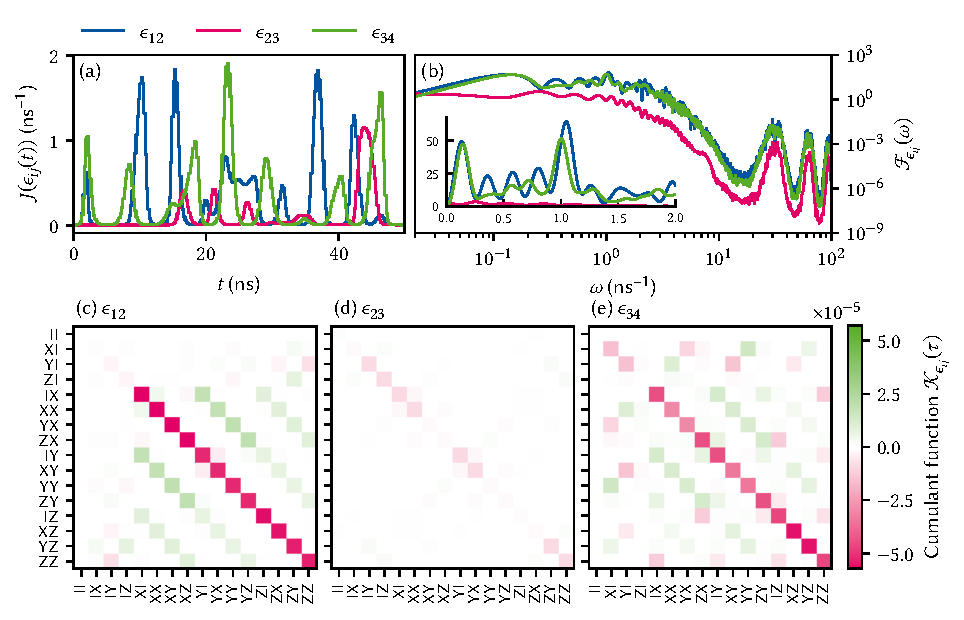
\includegraphics{img/pdf/filter_functions/CNOT_FF}
    \caption[\imgsource{img/py/filter_functions/cnot_FF.py}]{
        (a) Exchange interaction $J(\epsilon_{ij})$ for the \CNOT gate presented in~\citer{Cerfontaine2020b} as function of time.
        (b) Filter functions $\FF_{\epsilon_{ij}}$ for noise in the detunings evaluated on the computational subspace.
        The filter functions are modulated by oscillations at high frequencies due to numerical artifacts of the finite step size for the time evolution.
        The inset shows the filter functions in the DC regime on a linear scale with distinct peaks around $\omega = \flatfrac{2\pi}{\tau}$ and $\omega = \flatfrac{50}{\tau}$ ($\tau = \qty{50}{\nano\second}$).
        (c)--(e) Computational subspace block of the first order approximation of the error transfer matrix, given by the cumulant function $\cumulantfun_{\alpha\alpha}$ excluding second order contributions, for the \CNOT gate and the three detunings $\alpha\in\lbrace\epsilon_{12},\epsilon_{23},\epsilon_{34}\rbrace$.
        Note that in panel (e) the order of the rows and columns was permuted for better comparability.
    }
    \label{fig:ff:CNOT}
\end{figure*}

\Cref{fig:ff:CNOT} shows the filtered (convoluted) exchange interaction $J_{ij}$ between each pair of dots during the pulse sequence in panel (a) and filter functions plotted as function of frequency in panel (b) for the three different detunings.
For a detailed description on how the filter functions were computed in the presence of additional leakage levels refer to \cref{sec:app:ff:singlet-triplet}.
As one would expect from the fact that the intermediate (inter-qubit) exchange interaction $J_{23}$ (orange dash-dotted lines) is only turned on for short times to entangle the qubits, the filter function for $\eps_{23}$ is smaller by roughly an order of magnitude than the intra-qubit exchange filter functions.
Notably, the filter functions for $\eps_{12}$ and $\eps_{34}$ show clear characteristics of \glspl{dcg}, that is they drop to zero as $\omega\rightarrow 0$, and decouple from quasistatic noise with an error suppression $\propto\omega^2$.
This is not unexpected as the optimization minimizes quasistatic noise contributions to the infidelity.
In addition, one can also observe small oscillations with period $\qty{5}{\per\nano\second}$ in frequency space that arise as a numerical artifact of the piecewise constant discretization of the control parameters as investigations have shown.
If high-frequency spectral components are expected to play a significant role, one needs to be aware of these effects and adjust the simulation parameters appropriately.

The inset of \cref{fig:ff:CNOT}(b) shows the same filter functions for the DC tail on a linear scale.
Most notably, $\FF_{\epsilon_{12}}$ and $F_{\epsilon_{34}}$ have maxima around $\omega = \flatfrac{2\pi}{\tau}$, \ie exactly the frequency matching the pulse duration, and around $\omega = \flatfrac{50}{\tau} = \qty{1}{\per\nano\second}$ with $\tau_{\CNOT} = \qty{50}{\nano\second}$.
The former is the typical window in which a pulse is most susceptible to noise whereas the latter matches the absolute value of the magnetic field gradients, $b_{12} = -b_{34} = \qty{1}{\per\nano\second}$, indicating that the peak corresponds to the qubit dynamics generated by the magnetic field gradients.
Panels (c)--(e) show the cumulant functions $\cumulantfun_{\eps_{ij}}(\tau)$ of the detuning error channels $\eps_{ij}$ on the computational subspace.
$\cumulantfun_{\eps_{12}}$ displays clear characteristics of a Pauli channel with only elements on the diagonal and secondary diagonals deviating from zero significantly whereas $\cumulantfun_{\eps_{34}}$ (the target qubit) possesses a more complicated structure.

\begin{table}
    \centering
    \caption{
        Fast charge noise infidelity contributions to the total average gate fidelity of the two-qubit gate set from~\citer{Cerfontaine2020b} without capacitive coupling for GaAs \sts qubits compared to the original results.
        The fidelities are consistent with results from the reference within the uncertainty bounds of \qty{3}{\percent} of the Monte Carlo calculation.
        The infidelities presented here are all average gate infidelities (cf.
        \cref{eq:ff:fidelity:avg},~\citerr{Horodecki1999}{Nielsen2002}).
    }
    \label{tab:ff:infidelities}
    % This table is automatically generated by img/py/filter_functions/cnot_FF.py 
 \begin{tabularx}{\textwidth}{l *{4}{S[table-number-alignment=center,table-text-alignment=left,table-format=+1.1e+3,round-mode=figures,round-precision=2]}}
\toprule
 & \multicolumn{2}{c}{\textsc{This work}} & \multicolumn{2}{c}{\textsc{\citer{Cerfontaine2020b}}} \\
\cmidrule(lr){2-3}\cmidrule(lr){4-5}
$a$ & \sisetup{round-precision=1} 0 & \sisetup{round-precision=1} 0.7 & \sisetup{round-precision=1} 0 & \sisetup{round-precision=1} 0.7 \\
\midrule
\XID2 & 1.678739e-03 & 5.837005e-05 & 1.891736e-03 & 5.737387e-05 \\
\YID2 & 1.595312e-03 & 5.689787e-05 & 1.688837e-03 & 5.622157e-05 \\
\CNOT & 1.418439e-03 & 6.340114e-05 & 1.559636e-03 & 6.312606e-05 \\
\bottomrule
\end{tabularx}

\end{table}

We now compute the infidelity contribution originating from fast charge noise using \cref{eq:ff:fidelity:avg} but tracing only over the computational subspace to compare to the Monte Carlo calculations of~\citer{Cerfontaine2020b} (see \cref{sec:app:ff:singlet-triplet} for further details).
Like the reference, we use a noise spectrum $S_{\epsilon,a}(f)\propto \flatfrac{1}{f^a}$ with $S_{\epsilon,a}(\qty{1}{\MHz}) = \qty{4e-20}{\volt\squared\per\Hz}$ and consider white noise ($a = 0$) and correlated noise with $a = 0.7$~\cite{Dial2013} with infrared and ultraviolet cutoffs $\flatfrac{1}{\tau}$ and $\qty{100}{\per\nano\second}$, respectively.
\Cref{tab:ff:infidelities} compares the results in this work with the reference.
The values computed here are consistent with the more elaborate Monte Carlo calculations within a few percent.
Notably, the deviation is smaller for the smaller noise levels with $a = \num{0.7}$, in line with the fact that we have only computed the contributions from the decay amplitudes \decayamps and thus the leading order perturbation.
If we had additionally evaluated the frequency shifts \freqshifts we could have obtained the exact fidelity in the case of Gaussian noise.

\section{Rabi driving}\label{sec:ff:examples:rabi_driving}
A widely used method for qubit control is Rabi driving~\cite{Wallraff2004,Barends2014,Soare2014,Veldhorst2014}.
If we restrict ourselves to the resonant case for simplicity, the control Hamiltonian takes on the general form $\Hc = \flatfrac{\omega_0\sz}{2} + A\sin(\omega_0 t + \phi)\sx$.
Here, $\omega_0$ is the resonance frequency, $A$ the drive amplitude corresponding to the Rabi frequency in the weak driving limit $\flatfrac{A}{\omega_\mr{0}}\ll 1$, $\Omega_\mr{R}\approx A$, and $\phi$ an adjustable phase giving control over the rotation axis in the $xy$-plane of the Bloch sphere.
This Hamiltonian and associated decoherence mechanisms are well-studied in the weak driving regime, where the \gls{rwa} can be applied to remove fast-oscillating terms in the rotating frame~\cite{Jaynes1963,Gerry2008}.
There is a comprehensive understanding of how spectral densities transform to this frame and which frequencies are most relevant to loss of coherence~\cite{Yan2013}.

By contrast, the description of a system in the strong driving regime, where $\flatfrac{A}{\omega_0}\sim 1$, is more complicated since the \gls{rwa} cannot be applied without making large errors.
Yet, an improved understanding is desirable because strong driving allows for much shorter gate times and thus shifts the window of relevant noise frequencies towards higher energies where the total noise power is typically lower, \eg for \oneoverf noise.
Conversely, faster control also requires more accurate timing to prevent rotation errors.
It is therefore of interest to have available tools that can provide a comprehensive picture for Rabi pulses over a wide range of driving amplitudes.
By making use of the concatenation property of the filter functions, our formalism can do just that.

The problem that arises when trying to numerically investigate Rabi pulses in the weak driving regime in the lab frame is that typical control operations have a duration $\tau\gg T$ with $T = \flatfrac{2\pi}{\omega_0}$.
Since the sampling time step $\Delta t$ should additionally be chosen much smaller than a single drive period in order to sample the time evolution accurately ($\Delta t\ll T$), brute-force simulations are costly.

For $\flatfrac{T}{\Delta t} = 100$ samples per period and assuming Rabi and drive frequencies in typical regimes for \ch{SiGe} and \gls{mos} quantum dots~\cite{Zajac2018,Pla2012} or trapped ions~\cite{Soare2014}, $\Omega_\mr{R} = \qty{1}{\per\micro\second}$ and $\omega_0 = \qty{20}{\per\nano\second}$, a Monte Carlo simulation of a $\pi$-rotation with approximately \qty{3}{\percent} relative error would require $10^9$ samples in total.
Using the filter function formalism, we can drastically reduce the simulation time even beyond the improvement gained from concatenating precomputed filter functions of individual drive periods using \cref{eq:ff:control_matrix:sequence:freq}.
This can be achieved with \cref{eq:ff:control_matrix:sequence:periodic:simplified}, which simplifies the calculation of the control matrix for periodic Hamiltonians.

To benchmark our implementation, we use the parameters from above and calculate the control matrix of a NOT gate generated by a Rabi Hamiltonian with three different methods on an \fastprocessor.
First, we use \cref{eq:ff:control_matrix:sequence:freq} in a brute force approach.
Second, we utilize the concatenation property following \cref{eq:ff:control_matrix:pulse:freq:ff:calculation}.
Third, we employ the simplified expression given by \cref{eq:ff:control_matrix:sequence:periodic:simplified}.
The brute force approach takes \qty{250}{\second} of wall time whereas calculating the filter function using the standard concatenation is faster by two orders of magnitude, taking \qty{1.5}{\second} to run.
Lastly, the calculation utilizing the optimized method is faster again by two orders of magnitude and is completed in \qty{0.056}{\second}.

%\begin{table}[tbp]
%    \renewcommand\arraystretch{1.25}
%    %\setlength{\colwidth}{0.85 cm}
%    %\renewcommand\tabcolsep{0pt}
%    %\begin{tabular*}{\columnwidth}{l @{\extracolsep{\fill}} *{3}{S[table-number-alignment=center,table-text-alignment=center,round-mode=figures,round-precision=2]}}
%    \begin{tabular*}{\columnwidth}{@{\extracolsep{\fill}} *{4}{l}}
%    \toprule
%    Calculation method      & \cref{eq:ff:control_matrix:pulse:freq:ff:calculation}   & \cref{eq:ff:control_matrix:sequence:freq}    & \cref{eq:ff:control_matrix:sequence:periodic:simplified} \\
%    \colrule
%    %\midrule
%    Wall time (\unit{\second})& 370                                               & 1.3                                       & 0.079         \\
%    %Wall time (\unit{\second})& 367.4646                                          & 1.2895                                    & 0.0793       \\
%    %\bottomrule
%    \botrule
%    \end{tabular*}
%    \caption{Approximate wall times on an \fastprocessor for different ways of computing the control matrix of a Rabi-driven NOT gate with $10^6$ time steps and 500 frequency points highlighting the drastic performance improvement of using the optimized expressions.}
%    \label{tab:ff:rabi_driving:benchmark}
%\end{table}

As an example application, we calculate the filter functions for continuous Rabi driving in the weak and strong driving regimes.
For weak driving, we use the parameters from the benchmark above for a pulse of duration $\tau_\mr{weak}\approx\qty{20}{\micro\second}$ that corresponds to \num{20} identity rotations in total.
For the strong driving regime, we use the approximate analytical solution for a flux qubit biased at its symmetry point from~\citer{Deng2015} with $A = \flatfrac{\omega_0}{4}$ to drive the qubit for $\tau_\mr{strong}\approx\qty{4}{\nano\second}$ so that we achieve the same amount of identity rotations as in the weak driving case.
In the reference, strong driving in this regime is shown to give rise to non-negligible counterrotating terms that modulate the Rabi oscillations and which are well-described by Floquet theory applied to the Rabi driving Hamiltonian.
While for the regime studied here only two additional modes appear, the results extend to the regime where $A > \omega_0$ and up to eight different frequency components were observed.

\Cref{fig:ff:filter_function:rabi:weak_vs_strong} shows the filter functions $\FF_{xx}$ and $\FF_{zz}$ for the \sx and \sz noise operators in the weak (a) and the strong (b) driving regime.
Both display sharp peaks at their Rabi frequencies and the resonance frequency for $\FF_{zz}$ and $\FF_{xx}$, respectively.
We expect these features as they correspond to perturbations of the qubit Hamiltonian that are resonant with the qubit dynamics about an axis orthogonal to them.
For weak driving, $\FF_{xx}$ is constant up to the resonance frequency where it peaks sharply and then aligns with $\FF_{zz}$.
The latter has a peak at the Rabi frequency before rolling off with $\omega^{-2}$ and a DC level that is almost ten orders of magnitude larger than that of the transverse filter function.
This behavior is consistent with the results by~\citet{Yan2013}, who show that the noise sources dominating decoherence during driven evolution are $S_{xx}(\omega_0)$ and $S_{zz}(\Omega_\mr{R})$.
Note that the piecewise constant control approximation causes the weak driving filter functions to level off towards low frequencies after an initial roll-off (here at $\omega\sim\qty{1}{\per\milli\second}$).
By decreasing the discretization time step $\Delta t$, one can shift the frequency at which this effect occurs to lower frequencies and thus attribute the feature to a numerical artefact of the approximation.
However, the decoupling properties depend quite sensitively on the pulse duration.

In case of strong driving, the two filter functions are closer in amplitude for lower frequencies.
In addition, $\FF_{xx}$ also peaks at $\omega = \omega_0\pm\Omega_\mr{R}$.
These peaks also show up at higher frequencies in the dephasing filter function $\FF_{zz}$, reflecting frequency mixing in the strong coupling regime.
While both filter functions show characteristics of a \gls{dcg} in the weak driving regime, that is they drop to zero as $\omega\rightarrow 0$, this is not the case in the strong driving regime.
Instead, there they approach a constant level for small frequencies.
On top of rotation errors from timing inaccuracies, we may thus expect naive strong driving gates to be more susceptible to quasistatic noise than weak driving gates.
By shaping the pulse envelope of the strong driving gate the decoupling properties could be recovered.

\begin{figure*}
    \centering
    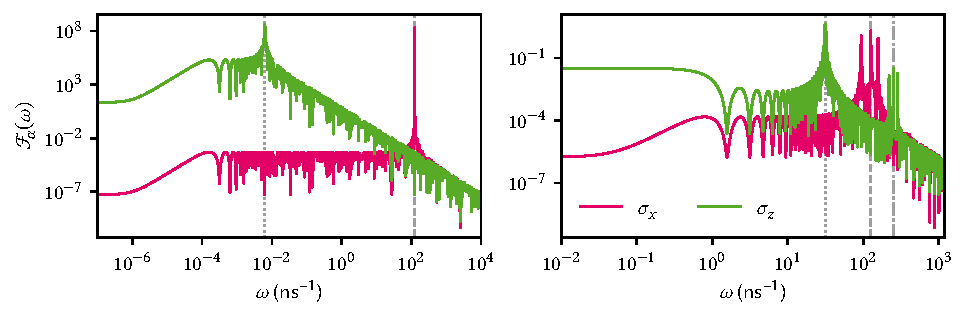
\includegraphics{img/pdf/filter_functions/rabi_driving_weak_vs_strong}
    \caption[\imgsource{img/py/filter_functions/periodic_driving.py}]{
        Filter functions for weak (a) and strong (b) Rabi driving (\num{20} identity gates in total).
        gray dashed (dotted) lines indicate the respective drive (Rabi) frequencies $\omega_0$ ($\Omega_\mr{R}$).
        (a) Weak driving with $\flatfrac{A}{\omega_\mr{0}}\ll 1$.
        The filter function $\FF_{xx}$ for noise operator \sx is approximately constant up to the resonance frequency where it peaks sharply and then aligns with the filter function $\FF_{zz}$ for \sz.
        $\FF_{zz}$ peaks at the Rabi frequency before rolling off with $\omega^{-2}$ and a DC level that is almost ten orders of magnitude larger than the DC level of the transverse filter function $\FF_{xx}$.
        (b) Strong driving with $\flatfrac{A}{\omega_\mr{0}}\sim 1$.
        Again $\FF_{zz}$ peaks at $\Omega_\mr{R}$ whereas $\FF_{xx}$ has three distinct peaks at $\omega_0$ and $\omega_0\pm\Omega_\mr{R}$.
        These features also appear at $2\omega_0$ in $\FF_{zz}$ due to the strong coupling (dash-dotted line).
    }
    \label{fig:ff:filter_function:rabi:weak_vs_strong}
\end{figure*}

\section{Randomized Benchmarking}\label{sec:ff:examples:randomized_benchmarking}
\Gls{srb} and related methods, for example \gls{irb}, are popular tools to assess the quality of a qubit system and the operations used to control it~\cite{Knill2008,Magesan2011,Magesan2012a}.
The basic protocol consists of constructing $K$ random sequences of varying length $m$ of gates drawn from the Clifford group,\sidenote{
    The Clifford group is a subgroup of the special unitary group with the advantage that compositions are easy to compute and that averaging over all unitaries can under reasonable assumptions be replaced by averaging over all Cliffords.
    This makes the Clifford gates a convenient choice for benchmarking.
    For a nice, short introduction as well as further references, see~\cite{Ozols2008}
}
and appending a final inversion gate so that the identity operation should be performed in total.
Each of these pulse sequences is applied to an initial state $\kpsi$ in order to measure the survival probability $p(\kpsi)$ after the sequence.
In reality, the applied operations are subject to noise and experimental imprecisions.
This renders them imperfect and results in a survival probability smaller than one.
Assuming gate-independent errors, the average gate fidelity $\avgfid$ is then obtained by fitting the measured survival probabilities for each sequence length to the zeroth-order exponential model~\cite{Magesan2011}
\begin{equation}\label{eq:ff:SRB}
p(\kpsi) = A \left(1 - \frac{dr}{d-1}\right)^m + B,
\end{equation}
where $r = 1 - \avgfid$ is the average error per single gate to be extracted from the fit, $A$ and $B$ are parameters capturing state preparation and measurement (SPAM) errors, and $d$ is the dimensionality of the system.

One of the main assumptions of the \gls{srb} protocol is that temporal correlations of the noise are small on timescales longer than the average gate time~\cite{Magesan2011}.
If this requirement is not satisfied, \eg if \oneoverf noise plays a dominant role, the decay of the sequence fidelity can have non-exponential components~\cite{Epstein2014,Fogarty2015,Feng2016} and a single exponential fit will not produce the true average gate fidelity~\cite{Mavadia2018,Edmunds2020}.
The filter function formalism suggests itself to numerically probe \gls{rb} experiments in such systems for two reasons.
First, it enables the study of gate performance subject to noise with correlation times longer than individual gate times.
This regime, where a simple description in terms of individual, isolated quantum operations fails, is accessible in the filter function formalism because universal classical noise can be included by the power spectral density $S(\omega)$.
Second, the simulation of a \gls{rb} experiment can be performed efficiently by using the concatenation property.
Because \gls{rb} sequences are compiled from a limited set of gates whose filter functions may be precomputed, one only needs to concatenate $m$ filter functions for a single sequence of length $m$ to gain access to the survival probability.

Since for sufficiently long \gls{rb} sequences $r\in\order{1}$, and we would need to include the frequency shifts \freqshifts in a full simulation following \cref{eq:ff:cumulant_expansion} because the low-noise approximation \cref{eq:ff:error_transfer_matrix:approx} does not hold in this regime.
Unfortunately, the concatenation property does not hold for \freqshifts.
Therefore, we focus on the high-fidelity regime where the exponential decay of the sequence fidelity may be approximated to linear order and only the decay amplitudes \decayamps need to be considered.

In order to evaluate the survival probability of a \gls{rb} experiment using filter functions, we employ the state fidelity from \cref{subsec:ff:theory:derived_quantities:state_fidelity-measurements} and focus on the single-qubit case with $d = 2$ and the (normalized) Pauli basis from \cref{eq:ff:basis:pauli}.
Because the ideal action of a \gls{rb} sequence is the identity we have $\liouvQ = \eye$.
Assuming we prepare and measure in the computational basis, $\kpsi\in\lbrace\ket{0}, \ket{1}\rbrace$ so that $\sqrt{2}\dket{\rho} = \dket{\sigma_0}\pm\dket{\sigma_3}$, we simplify \cref{eq:ff:fidelity:state} to
\begin{equation}\label{eq:ff:fidelity:state:RB}
\begin{split}
    \fid(\kpsi, \liouvU_\mr{RB}(\op{\psi})) &= \frac{1}{2}\bigl(\liouvUe_{00} +
    \liouvUe_{33}\pm
    \liouvUe_{03}\pm
    \liouvUe_{30}\bigr)
    = \frac{1 + \liouvUe_{33}}{2} \\
    &\approx 1 - \frac{1}{2}\sum_{k\neq 3}\decayamps_{kk}.
\end{split}
\end{equation}
For the second equality we used that \liouvUe is trace-preserving and unital (\cf \cref{subsec:ff:theory:transfer_matrix:derivation}) while in the last step we approximated the expression using \cref{eq:ff:error_transfer_matrix:approx,eq:ff:cumulant:truncated:liouville:pauli}.
For our simulation, we neglect SPAM errors so that $A =  B =  0.5$, choose $\kpsi = \ket{0}$, and approximate \cref{eq:ff:SRB} as
\begin{equation}\label{eq:ff:fidelity:state:RB:fit}
p(\ket{0}) = \fid(\ket{0}, \liouvU_\mr{RB}(\op{0}))\approx 1 - rm
\end{equation}
for small gate errors $r\ll 1$ since this is the regime which we can efficiently simulate using the concatenation property.

We simulate single-qubit \gls{srb} experiments using three different gate sets to generate the 24 elements of the Clifford group.
For the first gate set we implement the group by naive \enquote{single} rotations about the symmetry axes of the cube.
Each pulse corresponds to a single time segment during which one rotation is performed so that the $j$th element is given by $Q_j = \exp(-\i\phi_j\vec{n}_j\cdot\vec{\sigma})$.
We compile the other two gate sets from primitive $\flatfrac{\pi}{2}$ $x$- and $y$-rotations so that on average each Clifford gate consists of \num{3.75} primitive gates (see~\citer{Cerfontaine2020}).
For the specific implementation of the primitive $\flatfrac{\pi}{2}$-gates we compare \enquote{naive} rotations, \ie with a single time segment so that $Q_j = \exp-\i\pi\sigma_j/4)$ for $j\in\lbrace x, y\rbrace$, and the \enquote{optimized} gates from~\citer{Cerfontaine2020b}.
Pulse durations are chosen such that the average duration of all 24 Clifford gates generated from a single gate set is equal for all three gate sets.
This is to ensure that the different implementations of the Clifford gates are sensitive to the same noise frequencies.

We investigate white noise and correlated noise with $S(\omega)\propto\omega^{-0.7}$ assuming the same noise spectrum on each Cartesian axis of the Bloch sphere and normalize the noise power for each gate set and noise type (white and correlated) so that the average Clifford infidelity $r$ is the same throughout.
We then randomly draw $K = \num{100}$ sequences for \num{11} different lengths $m\in[1, 101]$ and concatenate the $m$ Clifford gates using \cref{eq:ff:control_matrix:sequence:freq} to compute the control matrix of the entire sequence.
For the integral in \cref{eq:ff:decay_amplitudes:freq} we choose the ultraviolet cutoff frequency two orders of magnitude above the inverse duration of the shortest pulse, $f_\mr{UV} = 10^2/\tau_\mr{min}$.
Similarly, the infrared cutoff is chosen as $f_\mr{IR} = 10^{-2}/m_\mr{max}\tau_\mr{max}$ with $m_\mr{max} = 101$ and $\tau_\mr{max} = 7\tau_\mr{min}$ (since the longest gate is compiled from seven primitive gates with duration $\tau_\mr{min}$) to guarantee that all nontrivial structure of the filter functions is resolved at small frequencies.\sidenote{
    For a precise fidelity estimate, the infrared cutoff should be extended to $f=0$.
    However, we are only interested in a qualitative picture and neglect this part of the spectrum here.
    At frequencies much smaller than $\approx\flatfrac{1}{\tau}$ where $\tau$ is the duration of the entire control operation, the filter function is constant and we therefore do not disregard any interesting features by setting $f_\mr{IR} = \flatfrac{10^{-2}}{\tau} = \flatfrac{10^{-2}}{m_\mr{max}\tau_\mr{max}}$.
}
%adequately.
Finally, we fit \cref{eq:ff:fidelity:state:RB:fit} to the infidelities computed for the different noise spectra.

The results of the simulation are shown in \cref{fig:ff:randomized_benchmarking:noise_comparison} (a) and (b) for white and correlated noise, respectively.
For white noise, the survival probability agrees well with the \gls{srb} prediction for all gate types whereas for \oneoverf-like noise the \enquote{single} gates (green pluses) deviate considerably.
Hence, fitting the zeroth-order \gls{srb} model to such data will not reveal the true average gate fidelity although errors are of order unity.
We note that~\citerr{Epstein2014}{Ball2016} found similar results using different methods for \oneoverf and perfectly correlated DC noise, respectively.
The former observed \gls{srb} to estimate $r$ within \qty{25}{\percent} and the latter found the mean of the \gls{srb} fidelity distribution to deviate from the mode, thereby giving rise to incorrectly estimated fidelities.

\begin{figure}[tbp]
    \centering
    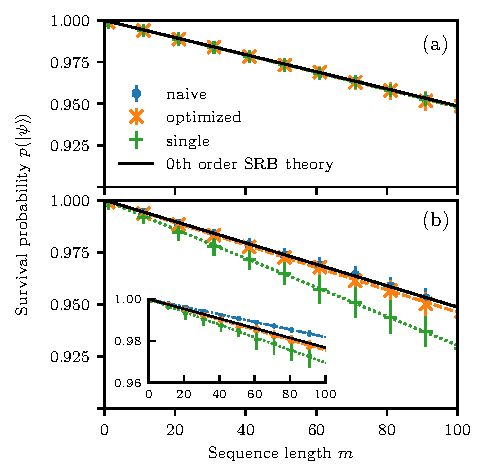
\includegraphics{img/pdf/filter_functions/RB_naive-optimized-single_gates_white_vs_correl_with_Z_noise_inset}
    \caption{
        Simulation of a \gls{srb} experiment using \num{100} random sequences per point for different gate and noise types (see the main text for an explanation of the gate type monikers).
        Dashed lines are fits of \cref{eq:ff:fidelity:state:RB:fit} to the data while the solid black lines correspond to a zeroth-order \gls{srb} model with $A=B=\num{0.5}$ and the true average gate infidelity per Clifford $r$.
        Errorbars show the standard deviation of the \gls{srb} sequence fidelities, illustrating that for the \enquote{single} gate set noise correlations can lead to amplified destructive and constructive interference of errors.
        The same noise spectrum is used for all three error channels (\sx, \sy, \sz) and the large plots show the sum of all contributions.
        (a) Uncorrelated white noise with the noise power adjusted for each gate type so that the average error per gate $r$ is constant over all gate types.
        No notable deviation is seen between different gate types.
        (b) Correlated \oneoverf-like noise with noise power adjusted to match the average Clifford fidelity in (a).
        The decay of the \enquote{single} gate set differs considerably from that of the other gate sets and the \gls{srb} decay expected for the given average gate fidelity, whereas \enquote{naive} and \enquote{optimized} gates match the zeroth order \gls{srb} model well, indicating that correlations in the noise affect the relation between \gls{srb} decay and average gate fidelity in a gate-set--dependent way.
        Inset: contributions from \sz-noise show that the sequence fidelity can be better than expected for certain gate types and noise channels.
    }
    \label{fig:ff:randomized_benchmarking:noise_comparison}
\end{figure}

On top of affirming the findings by the references, our results demonstrate that the accuracy of the predictions made by \gls{srb} theory, \ie that the \gls{rb} decay rate directly corresponds to the average error rate of the gates, not only depends on the gate implementation but also on which error channels are assumed.
This can be seen from the inset of \cref{fig:ff:randomized_benchmarking:noise_comparison}(b), where only dephasing noise (\sz) contributions are shown.
For this noise channel and the \enquote{naive} gates, one finds a slower \gls{rb} decay than expected from the actual average gate fidelity, so that the latter would be overestimated by an \gls{rb} experiment, whereas the \enquote{single} gates show the opposite behavior.
Depending on the gate set and relevant error channels, non-Markovian noise may thus even lead to improved sequence fidelities due to errors interfering destructively.
This behavior is captured by the pulse correlation filter functions whose contributions to the sequence fidelity lead to the deviations from the \gls{srb} prediction.

Notably, the data for the \enquote{optimized} gates agree with the prediction for every noise channel individually which implies that correlations between pulses are suppressed.
This highlights the formalism's attractiveness for numerical gate optimization as the pulse correlation filter functions $\FF\gth{gg^\prime}(\omega)$ may be exploited to suppress correlation errors.
To be more explicit, the correlation decay amplitudes $\decayamps\gth{gg^\prime}$ from \cref{eq:ff:decay_amplitudes:pulse_correlation} can be used to construct cost functions for quantum optimal control algorithms like \gls{grape}~\cite{Khaneja2005,Schulte-Herbruggen2005} or CRAB~\cite{Caneva2011}.
By constructing linear combinations of $\decayamps\gth{gg'}$ with different pulse indices $g$ and $g'$, correlations between any number of pulses can be specifically targeted and suppressed using numerical pulse optimization.

\section{Quantum Fourier transform}\label{sec:ff:examples:qft}
To demonstrate the flexibility of our software implementation, we calculate filter functions for a four-qubit \acrfull{qft}~\cite{Coppersmith1994,Nielsen2011} circuit.
The \gls{qft} routine plays an important role in many quantum algorithms such as Shor's algorithm~\cite{Shor1997} and quantum phase estimation~\cite{Nielsen2011}.
For the underlying gate set, we assume a standard Rabi driving model with IQ control and nearest neighbor exchange.
That is, we assume full control of the $x$- and $y$-axes of the individual qubits as well as the exchange interaction mediating coupling between two neighboring qubits.
This system allows for native access to the minimal gate set $\mathbb{G} = \lbrace\mr{X}_{i}(\flatfrac{\pi}{2}),\mr{Y}_{i}(\flatfrac{\pi}{2}),\mr{CR}_{ij}(\flatfrac{\pi}{2^3})\rbrace$ where $\mr{CR}_{ij}(\phi)$ denotes a controlled rotation by $\phi$ about $z$ with control qubit $i$ and target qubit $j$.
Controlled-$z$ rotations by angles $\flatfrac{\pi}{2^m}$ as required for the \gls{qft} can thus be obtained by concatenating $2^{3-m}$ minimal gates $\mr{CR}_{ij}(\flatfrac{\pi}{2^3})$.

Despite native access to all necessary gates, we employ \qutip's implementation~\cite{Johansson2012} of the \gls{grape} algorithm~\cite{Khaneja2005,Schulte-Herbruggen2005} to generate the gates in order to highlight our method's suitability for numerically optimized pulses.
For the optimization we choose a time step of $\Delta t = \qty{1}{\nano\second}$ and a total gate duration of $\tau = \qty{30}{\nano\second}$.
For completeness, see \cref{sec:app:ff:qft} for details on the optimized gates.
We then construct the remaining required gates by sequencing these elementary gates, \ie the Hadamard gate $\mr{H}_i = \mr{X}_{i}(\flatfrac{\pi}{2})\circ\mr{X}_{i}(\flatfrac{\pi}{2})\circ\mr{Y}_{i}(\flatfrac{\pi}{2})$, where $\mr{B}\circ\mr{A}$ denotes the composition of gates A and B such that gate A is executed before gate B .
To map the canonical circuit~\cite{Nielsen2011} onto our specific qubit layout with only nearest-neighbor coupling, we furthermore introduce SWAP operations to couple distant qubits.
These gates can be implemented by three \mr{CNOT}s, $\mr{SWAP}_{ij} = \CNOT_{ij}\circ\CNOT_{ji}\circ\CNOT_{ij}$.
The CNOTs in turn are obtained by a Hadamard transform of the controlled phase gate, $\CNOT_{ij} = \mr{H}_j\circ\mr{CR}_{ij}(\pi)\circ\mr{H}_j$.
The complete quantum circuit is shown at the top of \cref{fig:ff:qft}; for the canonical circuit with all-to-all connectivity refer to~\citer{Nielsen2011}.
In total, there are \num{442} elementary pulses, \num{198} of which are required for the three SWAPs on the first two qubits, so that the entire algorithm would take $\sim\qty{13}{\micro\second}$ to run.
Note that the circuit could be compressed in time by parallelizing some operations but for simplicity we only execute gates sequentially and do not execute dedicated idling gates.

\begin{figure*}
    %\resizebox{\columnwidth}{!}{}
    \centering
    \newcommand{\had}[0]{\gate{\mr{H}}}
\newcommand{\Rz}[1]{\gate{\mr{R}\!\left(\frac{\pi}{2^{#1}}\right)}}
\newcommand{\optX}{\gate{\mr{X}(\pi)}\gategroup[style={dashed,inner sep=0pt}]{}}

\begin{quantikz}[
    %thin lines,
    font=\footnotesize,
    column sep=1em,
]
    \lstick{3} &          & \optX    &          & \optX    &            & \ctrl{1} & \swap{1} &          & \optX    &          & \optX    &          &          &          &          &               & \permute{4,2,3,1} & \rstick{3} \\
    \lstick{2} &          &          &          & \ctrl{1} & \swap{1}   & \Rz{3}   & \targX{} &          &          &          & \ctrl{1} & \swap{1} &          &          &          & \permute{2,1} &                   & \rstick{2} \\
    \lstick{1} &          & \ctrl{1} & \swap{1} & \Rz{2}   & \targX{}   &          &          &          & \ctrl{1} & \swap{1} & \Rz{2}   & \targX{} &          & \ctrl{1} & \swap{1} &               &                   & \rstick{1} \\
    \lstick{0} & \had     & \Rz{1}   & \targX{} &          &            &          &          & \had     & \Rz{1}   & \targX{} &          &          & \had     & \Rz{1}   & \targX{} & \had          &                   & \rstick{0}
\end{quantikz}

    \bigskip
    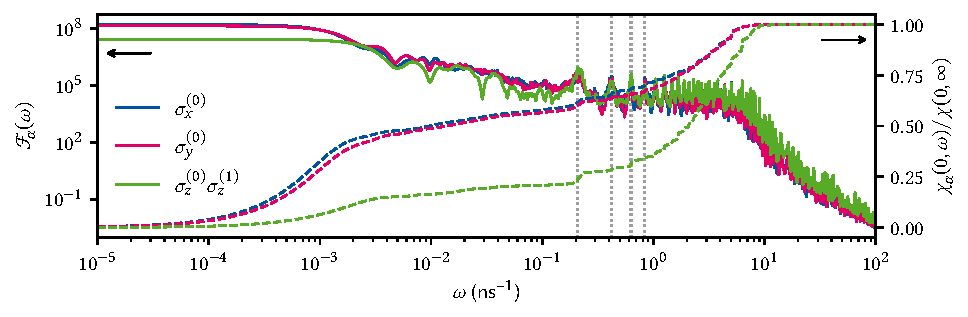
\includegraphics{img/pdf/filter_functions/qft_filter_function}
    \caption[\imgsource{img/tikz/circuits/qft.tex}\imgsource{img/py/filter_functions/quantum_fourier_transform.py}]{
        Top: Circuit for a \gls{qft} on four qubits with nearest-neighbor coupling.
        Labels next to the wires indicate the qubit index, showing that the final SWAP operation has already been carried out.
        Bottom: Filter functions for noise operators on the first qubit ($i = 0$).
        Dotted gray lines indicate the positions of the $n$ harmonic, $\omega_n = \flatfrac{2\pi n}{\tau}$ with $\tau = \qty{30}{\nano\second}$ the duration of the gates in $\mathbb{G}$, for $n\in\lbrace 1, 2, 3, 4\rbrace$.
        The filter functions have a baseline of around $10^4$ in the range $\omega\in[10^{-1}, 10^{1}]\,\unit{\per\nano\second}$ before they drop down to follow the usual $1/\omega^2$ behavior.
        The dashed lines show the error sensitivities $\chi_\alpha(\omega_1,\omega_2)\coloneqq\int_{\omega_1}^{\omega_2}\dd{\omega} \FF_\alpha(\omega)$ in the frequency band $[0, \omega]$ as a fraction of the total sensitivity $\chi_\alpha(0,\infty)$.
        These are closely related to the entanglement fidelity (\cf \cref{eq:ff:filter_function:fidelity,eq:ff:infidelity:ent:integral}) and suggest that high frequencies up to the knee at $\omega\approx\qty{10}{\per\nano\second}$ cannot be neglected if the cutoff frequency of the noise is sufficiently high or the spectrum does not drop off quickly enough (note the linear scale as opposed to the logarithmic scale for the filter functions).
    }
    \label{fig:ff:qft}
\end{figure*}

In order to leverage the extensibility of the filter function approach (see \cref{sec:ff:performance:extending_hilbert_spaces}), we use a Pauli basis for the pulses and proceed as follows:
\begin{enumerate}
    \item Instantiate the \pulsesequence objects for the elementary gates $\mathbb{G}$ for the first two qubits and cache the control matrices.
    \item Compile all required single- and two-qubit pulses by concatenating the \pulsesequences that implement $\mathbb{G}$.
    \item Extend the \pulsesequences to the full four-qubit Hilbert space.
    \item Recursively concatenate recurring gate sequences by concatenating four-qubit \pulsesequences, \eg $\mr{SWAP}_{10}\circ\mr{CR_{10}}(\flatfrac{\pi}{2^1})\circ\mr{H}_0$, in order to optimally use the performance benefit offered by \cref{eq:ff:control_matrix:sequence:freq}
    \item Concatenate the last \pulsesequences to get the complete \gls{qft} pulse.
\end{enumerate}
For our gate parameters and \num{400} frequency points, this procedure takes around \qty{5}{\second} on an \fastprocessor, whereas computing the filter functions naively using \cref{eq:ff:control_matrix:pulse:freq:ff:calculation} takes around \qty{4}{\minute}.
The resulting filter functions are shown in \cref{fig:ff:qft} for the noise operators affecting the first qubit; for an in-depth discussion and validation of the fidelities predicted, see the accompanying letter~\citer{Cerfontaine2021} and its supplementary information.
Evidently, the fidelity of the algorithm is most susceptible to DC noise; below roughly $\omega\lessapprox 10^{-3}\,\unit{\per\nano\second}$ the filter functions level off at their maximum value.
In the \unit{\giga\hertz} range there is a plateau with sharp peaks corresponding to the $n$ harmonics of the inverse pulse duration $\omega_n = \flatfrac{2\pi n}{\tau}$, where the leftmost belongs to $n=1$.
The dashed lines show the error sensitivities $\chi_\alpha(\omega_1, \omega_2)\coloneqq\int_{\omega_1}^{\omega_2}\dd{\omega}\FF(\omega)$ in the frequency band $[0, \omega]$ relative to the total sensitivity $\chi_\alpha(0,\infty)$.
For a white spectrum, \ie $S(\omega)=\mr{const.}$, this quantifies the fraction of the total entanglement infidelity that is accumulated up to frequency $\omega$ (\cf \cref{eq:ff:filter_function:fidelity,eq:ff:infidelity:ent:integral}).
Thus, to obtain a precise estimate of the algorithm's fidelity, five frequency decades need to be taken into account.

These insights demonstrate that our method represents a useful tool to analyze how and to which degree small algorithms are affected by correlated errors, and how this effect depends on the gate implementation.
It could thus also be used to choose or optimize gates in an algorithm-specific way.

